\section{Binary Decision Diagram}

The core idea behind ROBDDs is to avoid the inefficiencies of sequential sub-case exploration by instead storing sub-cases in memory, allowing for faster retrieval and processing.
This approach relies on two crucial hashing mechanisms: a unique table and a computed table. 
The unique table identifies and consolidates identical sub-cases to prevent redundancy, while the computed table stores the results of previously computed sub-cases to reduce redundant calculations.

ROBDDs represent logic functions as Directed Acyclic Graphs (DAGs), which often provide a more compact form than traditional Sum of Products (SOP) expressions. 
With careful structuring, ROBDDs can be made canonical, meaning they provide a unique representation of a function. 
This can shift the focus in Boolean reasoning from solving SAT problems to efficiently managing function representation.

Another significant advantage is the efficiency of Boolean operations on BDDs. 
Many operations, such as checking for tautology or computing complements, can be performed quickly—often in linear time relative to the result's size or even in constant time. 
However, the size of a BDD is critically influenced by variable ordering, with the right orderings resulting in significantly smaller, more manageable diagrams.

\paragraph*{Directed Acyclic Graph representation}
In an ROBDD, the logic function is represented by a Directed Acyclic Graph (DAG) with a structure rooted in a single root node and terminating in two terminal nodes, labeled 0 and 1. 
Each internal node in the graph is associated with a variable and has exactly two children. 
The DAG's structure is based on a Shannon co-factoring tree, modified to be both reduced and ordered, creating the canonical form known as ROBDD: 
\begin{itemize}
    \item \textit{Reduction}: this process simplifies the graph by eliminating redundancy: if a node has two identical children, it is removed, else if two nodes have identical subgraphs, they are merged into a single node.
    \item \textit{Ordering}: co-factoring (splitting) variables are processed in a consistent, predefined order across all paths, ensuring that each path from the root to any terminal visits variables in ascending order, typically denoted $x_1<\dots<x_n$.
\end{itemize}

An Ordered Binary Decision Diagram (OBDD) applies only the ordering rule, while a Reduced Ordered Binary Decision Diagram (ROBDD) applies both ordering and reduction. 
The ROBDD's reduction rules are:
\begin{enumerate}
    \item If a node's two children are identical, the node is removed, effectively reducing the function to $f = vf + \bar{v}f$. 
    \item If two nodes have isomorphic graphs, they are replaced by a single instance, so each node uniquely represents a distinct logic function.
\end{enumerate} 
The onset of the function represented by an ROBDD can be identified by tracing all paths leading to the 1-terminal node. 
This set of paths corresponds to a cover of pairwise disjoint cubes, providing an efficient and compact representation of the function without needing to explicitly enumerate every path.

\subsection{Implementation}
The BDD can be implemented via: 
\begin{itemize}
    \item \textit{Unique table}: prevents duplication by ensuring that each node in the BDD is unique.
        Implemented as a hash table, where each node's properties (key) map to an existing or new node (value).
    \item \textit{Computed table}: stores results of previously computed operations, avoiding redundant calculations.
\end{itemize}
BDDs represent a compressed form of the Shannon co-factoring tree:
\[f=vf_v+\bar{v}f_{\bar{v}}\]
where the leaf nodes are constants, either 0 or 1.

To maintain a canonical form, ROBDDs follow three rules (as demonstrated by Bryant in 1986):
\begin{enumerate}
    \item Unique nodes for constants 0 and 1.
    \item Consistent ordering of decision variables along all paths.
    \item Use of a hash table that ensures:
        \[(\text{node}(f_v) = \text{node}(g_v)) \land (\text{node}(\bar{f}_v) = \text{node}(\bar{g}_v)) \implies \text{node}(f) = \text{node}(g)\]
        This ensures uniqueness of $\text{node}(f)$ using the unique hash table.
\end{enumerate}
The order of variables is fixed, so if $v < w$, then $v$ appears higher in the ROBDD structure.
The top variable associated with the root node of $f$ becomes the key variable for subsequent operations.


\subsection{If-then-else operator}
The ITE operator can implement any two-variable logic function, representing 16 possible operations (all subsets of $B^2$): 
\[\text{ite}(f,g,h)=fg+f\bar{h}\]

\paragraph*{Unique hash table}
Before adding a new node $(v, g, h)$ to the BDD, the unique table is checked to ensure it doesn't duplicate an existing node.
If a match exists, the existing node pointer is reused; otherwise, a new node is added to the table.
This process maintains the BDD's canonical form, ensuring that a node $(v, g, h)$ exists in the unique table if and only if it has been explicitly added. 
Thus, there's only one pointer to each unique table entry, supporting multi-rooted Directed Acyclic Graphs (DAGs) for multiple functions.
\begin{algorithm}[H]
    \caption{Recursive ITE}
    \begin{algorithmic}
        \Function{ITE}{$f, g, h$}
            \If{$f == 1$} 
                \State \Return $g$
            \EndIf
            \If{$f == 0$} 
                \State \Return $h$
            \EndIf
            \If{$g == h$} 
                \State \Return $g$
            \EndIf
            \If{$p =$ \Call{HashLookupComputedTable}{$f, g, h$}} 
                \State \Return $p$
            \EndIf
            \State $v=$ \Call{TopVariable}{$f,g,h$}
            \State $fn=$ \Call{ITE}{$f_v, g_v, h_v$}
            \State $gn=$ \Call{ITE}{$f_{\bar{v}}, g_{\bar{v}}, h_{\bar{v}}$}
            \If{$fn == gn$} 
                \State \Return $gn$
            \EndIf
            \If{$!(p =$ \Call{HashLookupComputedTable}{$v, fn, gn$})}
                \State $p=$ \Call{CreateNode}{$v, fn, gn$}
                \State Insert $p$ into the unique table
            \EndIf
            \State $key=$ \Call{HashKey}{$f, g, h$}
            \State \Call{InsertComputedTable}{$p,key$}
            \State \Return $p$
        \EndFunction
    \end{algorithmic}
\end{algorithm}

\subsection{Computed table}
The computed table stores triplets of the form $(f,g,h)$ representing results already computed by the ITE operator.
Implemented as a software cache, this table reduces redundant calculations and improves efficiency. 
To facilitate rapid lookups, the computed table uses a hash table designed as a lossy cache without collision handling chains.

\paragraph*{Complemented edges}
Complemented edges allow the BDD to represent inverted functions efficiently, reducing memory usage and accelerating operations like NOT and ITE. 
This structure is similar to optimizations in circuit design. 
However, to maintain the strong canonical form of the BDD, four edge equivalences must be managed, ensuring consistent representation across nodes. 
\begin{figure}[H]
    \centering
    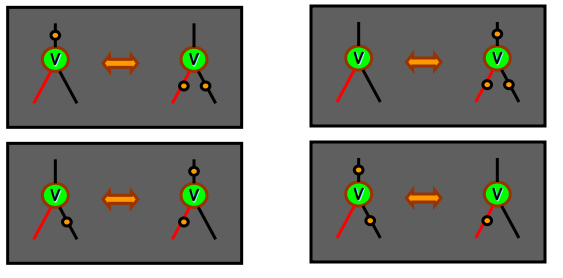
\includegraphics[width=0.75\linewidth]{images/ed1.png}
    \caption{Ege equivalences}
\end{figure}
The preferred convention is to position the complement-free edge on the left (or “then” leg) of the structure.

\paragraph*{Optimization}
To maximize successful matches in the computed table, the following conventions are typically observed:
\begin{enumerate}
    \item The first argument is chosen based on the smallest top variable to maintain a predictable order.
    \item When variables are tied, the smallest address pointer is chosen, though this can sometimes limit portability.
\end{enumerate}
Efficient BDD operations require caching mechanisms:
\begin{itemize}
    \item \textit{Local cache}: temporary storage for single operations, which is cleared after the operation completes.
    \item \textit{Operation-specific cache}: dedicated caches for specific operations to reduce the need for type-tracking.
    \item \textit{Shared cache}: a universal cache for all operations, improving memory management but requiring storage of operation types.
\end{itemize}

\subsection{Garbage collection}
Effective garbage collection is crucial for managing memory in BDDs, as unused nodes consume resources. 
BDD nodes can be deallocated by external \texttt{bdd\_free} operations for nodes that are no longer referenced externally or by reclaiming nodes created temporarily during BDD operations.
Mechanisms to Detect Unreferenced Nodes

\paragraph*{Unreferenced nodes}
\begin{enumerate}
    \item \textit{Reference counting}: each node maintains a counter that increments when a new reference is created and decrements when a reference is removed. 
        If a counter overflows, the node freezes and remains in memory.
    \item \textit{Mark-and-sweep algorithm}: this method, which doesn't rely on reference counts, marks all referenced BDD nodes in a first pass and frees unmarked nodes in a second pass. 
        An external reference handle layer may be needed for accuracy.
\end{enumerate}

\paragraph*{Timing}
Since garbage collection can be resource-intensive, its timing is critical. 
Options include:
\begin{itemize}
    \item \textit{Immediate deallocation}: freed nodes are reclaimed right away, though this approach risks reallocation in the next operation.
    \item \textit{Scheduled collections}: regular garbage collection can be triggered based on statistics gathered during BDD operations.
    \item \textit{Death row retention}: nodes are temporarily retained before final deletion to improve reuse in subsequent operations.
\end{itemize}
Because computed tables don't use reference tracking, they must be cleared independently during garbage collection.
Sorting freed nodes also improves memory locality, enhancing cache performance and overall efficiency.